\section{Image acquisition and phenotyping}
The cohort used for the genetic association study of left ventricular trabeculation consists of the samples with European ancestry that passed the genotyping and imputation quality control described in \cref{subsection:genotypes}. Since there is no ground to suspect confounding of the phenotype processing based on the relatedness of samples as it was the case in the previous chapter (\cref{chapter:GWAS-3Dheart}), related samples were included in the cohort. For each of the \num{1207} samples, the level of trabeculation was measured at six to ten positions in the heart. Trabeculation was quantified via fractal analysis, a technique which allows to measure the complexity of patterns \citep{Eke2002}. Fractal analysis yields a unit-less measure, the \gls{fd}, which quantifies the complexity of the analysed structure. The higher the \gls{fd} measure, the higher the complexity of the structure i.e. the more trabeculation is observed in the left ventricular wall. 

The pipeline for the automatic detection and quantification of trabeculation in the left ventricle was developed by Jiashen Cai and Pawel Tokarczuk. In the following paragraph, I briefly describe the image acquisition and phenotype extraction procedure. 

2D cardiac magnetic resonance imaging was conducted at the Hammersmith Hospital, London. The fractal dimensions were derived from standard left ventricular short axis 2D cardiac magnetic resonance images in the plane from base to apex. Each section had a thickness of \num{8}~mm with a \num{2}~mm gap between sections. A more detailed description of the imaging parameters can be found in \citep{deMarvao2014}. Fractal analysis was automated according to the protocol proposed by Captur and colleagues \citeyearpar{Captur2013}. First, the images (\cref{fig:scheme-fd}, \subfig{1}) were binarised into blood pool and myocardium (\cref{fig:scheme-fd}, \subfig{2}) and the endomyocardial border extracted via edge detection (\cref{fig:scheme-fd}, \subfig{3}). The \gls{fd} was determined by placing grids with known spacing (scale) of increasing size (i.e. increasing number of edges) on the image and subsequent counting of the number of boxes with non-zero pixels, i.e. how many boxes contain at least one pixel of the border (\cref{fig:scheme-fd}, \subfig{4}). The slope of the linear regression of the ln-transformed scale versus the ln-transformed counts corresponds to the \gls{fd} (\cref{fig:scheme-fd}, \subfig{5}) \citep{Captur2013}.

\begin{figure}[hbtp]
	\centering
	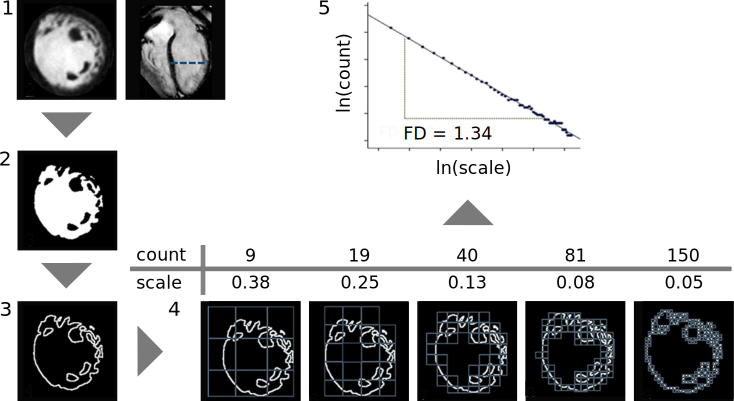
\includegraphics[trim = 0mm 0mm 0mm 0mm, clip, width=\textwidth]{Chapter6/Figures/FD_scheme.pdf}
	\caption[\textbf{FD phenotyping scheme. }]{\textbf{FD phenotyping scheme. }\gls{fd} is determined for each of the left ventricular short axis slices derived from standard 2D cardiac magnetic resonance images. 1. An example left ventricular short axis slice is depicted on the left, its location in the heart is indicated by the dashed line of the heart image on the right. 2. The image is binarised into blood pool (white) and other structures (black). 3. The border between the white and the black background is the endocardial wall, which can be extracted via edge detection. 4. A standard box-counting method is applied to the image of the extracted border, where grids of known spacing (scale) are placed on top of the image and boxes containing at least one pixel of endocardial borders are counted. 5. The slope of the regression of the ln-transformed scale versus the ln-transformed count is the \gls{fd}. Adapted from \citep{Captur2013}.} 
	 	\label{fig:scheme-fd}
\end{figure}

\section{The complexity of trabeculation shows a consistent base to apex pattern}
For \num{1192} out of the \num{1207} genotyped samples, \gls{fd} measurements could successfully be computed at each slice. Their distribution from base to apex is depicted in \cref{fig:perslice-fd}. Both at the tip of the apex and the end of the basal zone, \gls{fd} is generally lowest and increases towards the mid-section of the heart. Similar results have been observed by \citep{Kawel2012} and \citep{Captur2014}. The latter have shown that most variation between healthy and diseased individuals exists in \gls{fd} measurements derived from the apical slices of the heart ( \cref{fig:perslice-fd}\subfig{A}) and used the maximal \gls{fd} value observed in these slices as their final phenotype. I followed the strategy of dividing the measurements into apical and basal (\cref{fig:perslice-fd}\subfig{B}) and used the maximum \gls{fd} observed in each group as final phenotypes. For individuals with uneven numbers of slices, the center slice was not considered for the computation of the maximum values.
\\
\begin{figure}[hbtp]
	\centering
	\includegraphics[trim = 0mm 0mm 0mm 0mm, clip, width=\textwidth]{Chapter6/Figures/FDalongHeart.pdf}
	\caption[\textbf{FD measurements from base to apex. }]{\textbf{FD measurements from base to apex. } A. Location of the 2D cardiac magnetic resonance image slices and their classification into apical and basal. B. FD measurements for all samples were interpolated via a cubic spline function to the maximum number of \num{10} slices for easier visualisation. Subsequent analyses were done based on the original, non-interpolated FD measurements.} 
	 	\label{fig:perslice-fd}
\end{figure}

\section{Relationship between trabeculation phenotypes and covariates}
\begin{figure}[hbtp]
	\centering
	\includegraphics[trim = 0mm 0mm 0mm 0mm, clip, width=\textwidth]{Chapter6/Figures/pairs_fdcovariates.pdf}
	\caption[\textbf{Relationship between FD measures and covariates. }]{\textbf{Relationship between FD measures and covariates. }Continuous variables: the univariate-distribution of each variable is depicted on the diagonal. The upper triangular matrix shows the bi-variate distribution while the lower triangular matrix shows the regression line of their linear fit. Categorical variables (sex): Distribution (first row) and counts (first column) are depicted. } 
	 	\label{fig:covariates-FD}
\end{figure}

I analysed the distribution of the \num{2} \gls{fd} measurements  \(\text{FD}_\text{max}^\text{basal}\) and \(\text{FD}_\text{max}^\text{apical}\) in relation to biological and cardiac covariates (\cref{fig:covariates-FD}). Both \gls{fd} measurements show correlation with age, weight and left ventricular mass.   \(\text{FD}_\text{max}^\text{basal}\) is additionally associated with height, while \(\text{FD}_\text{max}^\text{apical}\) also shows correlation with sex (\cref{tab:covariates-FD}). The association of\gls{lvm} and \(\text{FD}_\text{max}^\text{apical}\)  confirms the findings of the study by Captur and colleagues \citep{Captur2014}, who found increased \gls{fd} measures for individuals with increased \gls{lvm}. However, the causality of the relationship has not been determined yet. All associated covariates except for \gls{lvm}, as the causal relationship to \gls{fd} measurements is unclear, were used as covariates in the \gls{gwas}. 

% Table generated by Excel2LaTeX from sheet 'FDCovariates'
\begin{table}[htbp]
  \centering
  \caption[\textbf{Association of \(\text{FD}_\text{max}^\text{basal}\) and \(\text{FD}_\text{max}^\text{apical}\) with covariates. }]{\textbf{Association of \(\text{FD}_\text{max}^\text{basal}\) and \(\text{FD}_\text{max}^\text{apical}\) with covariates. } Association was determined based on a simple linear model for each \gls{fd} measurement with all covariates as explanatory variables without interaction effects.}
    \begin{tabular}{lll}
    \toprule
          &  \(\text{FD}_\text{max}^\text{basal}\) & \(\text{FD}_\text{max}^\text{apical}\) \\
    \midrule
    Sex   & \num{5.47E-01} & \num{4.96E-03} \\
    Age   & \num{3.04E-08} & \num{2.87E-04} \\
    Height & \num{4.33E-02} & \num{4.43E-01} \\
    Weight & \num{1.25E-04} & \num{4.55E-05} \\
    \gls{lvm}   & \num{1.21E-12} & \num{2.62E-03} \\
    Slices & \num{8.02E-01} & \num{3.89E-01} \\
    \bottomrule
    \end{tabular}%
  \label{tab:covariates-FD}%
  \vspace{-2mm}
\end{table}%